%% ID: space_monster_attack
%% TITLE: Space monster attack
%% TYPE: question
%% QUESTIONTYPE:  numerical
%% CONCEPTS: forces, newtoni, newtonii, moments
%% VIDEOS: 
%% LEVEL: 5
%% TOPIC: mechanics/statics
%% ORDER: 9

\begin{problem}[Zephyr_Space_Monster_Attack]%FRes, CoM, MomRes, Trig, Calculus %USED
{
\begin{enumerate}
	\item \question[a]{By considering a triangle as a collection of infinitesimally small rectangles, show that the centre of mass of a lamina in the shape of a right-angled triangle, resting on it's shortest side, is a third of the height from the base.}
	\item \question[b]{Hence find the position of the centre of mass of any triangle which is symmetric in a line that passes through it's base.}
	\item \question[c]{The spaceship shown in Figure \ref{fig:Statics_spaceship} consists of four sections, a square bridge, two sets of rectangular living quarters and a triangular engine bay. The engine bay is twice as dense as the other parts of the ship. Find the position of the centre of mass of the ship given $a = 3b$.
	\begin{figure}[h]
	\centering
	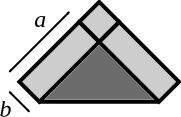
\includegraphics[width=0.5\textwidth]{../../../figures/Statics_spaceship.svg}
	\caption{}
	\label{fig:Statics_spaceship}
\end{figure}}
	\item \question[d]{These spaceships are designed so they can dock together in a fleet of four, as shown in Figure \ref{fig:Statics_spaceship_docking}. Unfortunately whilst docked the fleet floats close to an asteroid on which lurks a ravenous Bugblatter Beast of Traal. The beast swallows one of the ships whole leaving the formation looking like Figure (\ref{fig:Statics_spaceship_attacked}). Find the centre of mass of the remaining fleet.
	\begin{figure}[h]
	\centering
	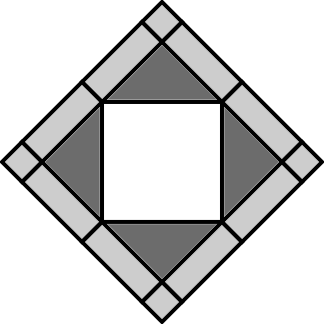
\includegraphics[width=0.4\textwidth]{../../../figures/Statics_spaceship_docking.svg}
	\caption{}
	\label{fig:Statics_spaceship_docking}
\end{figure}

\begin{figure}[h]
	\centering
	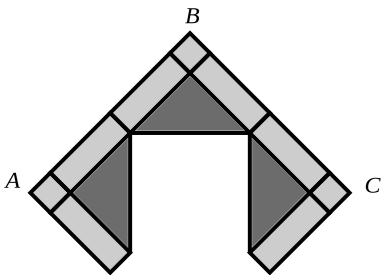
\includegraphics[width=0.4\textwidth]{../../../figures/Statics_spaceship_attacked.svg}
	\caption{}
	\label{fig:Statics_spaceship_attacked}
\end{figure}}

	\item \question[e]{In an attempt to stop the other ships escaping the Bugblatter Beast disables the main engines of the remaining ships using it's electrified tentacles. Unbeknownst to it though, each of the ships has a tiny docking engine at the front tip of the bridge. The beast grabs the bridges of ships $A$ and $C$, on their very corners and pulls them in equal and opposite vertical directions, trying to rip the ships apart with it's two monstrous heads.
	
	The ships docking engines can point in any direction, and the captain knows that if she can ensure the ship does not rotate then the beast will get confused and forget about it's quarry. Assuming the engines can produce exactly enough force to save the crew if pointed in the right direction, which directions should they point in order to confuse the beast?}
	
	%Thought the question was long enough by this point, but this could be added in too?
	%Given that the Bugblatter Beast has three sets of jaws on each head, and each set can produce 100 N of force and the coefficient of friction between it's teeth and the spaceship is 0.5, will the ships engine's, each producing 100 N of thrust, be sufficient to confuse the beast?
\end{enumerate}
}
{Written by Zephyr Penoyre for the RSPP}
{\answer[a]{}
\answer[b]{}
\answer[c]{}
\answer[d]{}
\answer[e]{}
\begin{enumerate}
\begin{figure}[h]
	\centering
	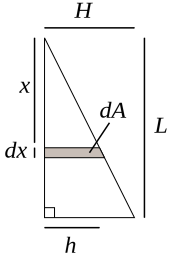
\includegraphics[width=0.4\textwidth]{Statics_spaceship_triangle}S
	\caption{}
	\label{fig:Statics_spaceship_triangle}
\end{figure}

	\item We know that around any point, the moment produced is equal to the distance to that point $X$ multiplied by the force due to the total mass $M$. This must also be equal to the sum of the moment of each individual section of the shape. Examining Figure (\ref{fig:Statics_spaceship_triangle}) we can see how we can split the original triangle up into small segments with area $d{A}$ and thus mass $dm =\rho~ d{A}$ where $\rho$ is the density.
	
	As the triangle defined by $x$ and $h$ must be similar to that defined by $L$ and $H$, we know $h = \frac{Hx}{L}$.
	
	For small enough $d{x}$, the area $d{A}$ can be approximated as a rectangle, thus:
	
	\begin{equation}	d{A} = h~d{x} = \frac{H x~d{x}}{L}  \end{equation}
	
	Total moment $G$, taken around the point $x=0$, satisfies:
	
	\begin{equation}	G = M X = \sum{x~dm} = \sum{\frac{\rho H x^{2} ~dx}{L}}  \end{equation}
	
	As $dx$ goes to zero the sum of finite areas $dA$ goes to a continuous integral:
	
	\begin{equation}	G = \int_0^L \frac{\rho H x^2}{L}~ \d{x} = \frac{\rho H}{L}\left[\frac{x^3}{3}\right]^L_0 = \frac{\rho H L^2}{3}  \end{equation}
	
	Also we know $M = \rho A = \rho \frac{H L}{2}$
	
	And therefore:
	
	\begin{equation}	 \rho \frac{H L}{2} D =  \frac{\rho H L^2}{3} 
	 \Rightarrow D = \frac{2L}{3} \end{equation}
	
	Thus the centre of mass lies two thirds of the distance from the tip, and thus one third of the distance from the base.
	
	\item Any triangle that is symmetrical through it's base can simply be thought of as two right-angled triangles, such as those in Figure (\ref{fig:Statics_spaceship_triangle}), placed back to back.
	
	Thus the horizontal components of the position of the centre of mass, relative to the line of symmetry, are equal and opposite and cancel out.
	
	The vertical components of both triangles centre of mass positions are the same and thus the distance of the c.o.m. from the base must be unchanged.
	
	Thus the centre of mass sits on the line of symmetry, one third of the height above the base.
	
	\item
	
	As the ship has a vertical line of symmetry we know it's c.o.m. must sit on this line. Defining the vertical distance, from the base, to the centre of the bridge as $x\s{1}$, to the centre of the living quarters as $x\s{2}$ and to the c.o.m of the engine bay as $x\s{3}$ (for the other parts of the ship the centre and the c.o.m. are equivalent)
	
	It is easy to deduce that the angles at the base of the triangle are both $45^{\circ}$ and as $\sin{45^{\circ}} = \frac{1}{\sqrt{2}}$ the height of the triangle $H = \frac{a}{\sqrt2}$ and thus $x\s{3} = \frac{H}{3} = \frac{a}{3\sqrt{2}}$.
	
	\begin{equation}	x\s{1} = \frac{a}{\sqrt{2}} +  \frac{b}{2\sqrt{2}} \end{equation}
	
	and
	
	\begin{equation}	x\s{2} = \frac{a}{2\sqrt{2}} +  \frac{b}{2\sqrt{2}} \end{equation}
	
	Can take the density of the bridge and living quarters as 1 without loss of generality. Thus the mass of the bridge $M\s{1} = b^2)$ and the mass of a single living quarter, $M\s{2} = ab$. Remembering that the density of the engine bay is twice that of the rest of the ship, it's mass $M\s{3} = 2(\frac{a^2}{2}) = a^2$.
	
	If we label the distance from the base to the c.o.m. as $D$ and total mass as $M$:
	
	\begin{equation}	M D = (b^2 + 2ab + a^2) D = (a + b)^2 D = b^2 \left( \frac{a}{\sqrt{2}} +  \frac{b}{2\sqrt{2}} \right) +  2ab \left( \frac{a}{2\sqrt{2}} +  \frac{b}{2\sqrt{2}} \right) +  a^2 \left( \frac{a}{3\sqrt{2}} \right)\end{equation}
	
	Substituting in $a = 3b$ and rearranging we find:
	
	\begin{equation} D = \frac{25b}{16\sqrt{2}} \end{equation}
	
	\item
	
	With three ships connected together we can examine the c.o.m. position relative to the middle ship, such that the formation is symmetric and thus we know the c.o.m will lie on that line.
	
	Redefining $M$ as the total mass of the three ships, each of mass $m~ (= 16 b^2)$, and $D$ as the distance of the c.o.m. relative to the centre of the square made by four ships in formation, where the base of each ship is a distance $\frac{a}{\sqrt2} = \frac{3b}{\sqrt2}$ from this point. Only the middle ship has a component of it's position in the direction of $D$, thus:
	
	\begin{equation} M D = 3 m D = m \left(  \frac{3b}{\sqrt2} +  \frac{25b}{16\sqrt{2}} \right) \end{equation}
	
	\begin{equation}\Rightarrow D = \frac{1}{3} \left( \frac{73 b}{16\sqrt{2}} \right) = \frac{73b}{48\sqrt{2}} \end{equation}
	
	\item
	
	The maximum moment can be produced by the engines by pointing perpendicularly away from the centre of mass. Thus the engine at B must point horizontally, whilst the engines at A and C must point at angle $\theta$ from the vertical, satisfying:
	
	\begin{equation} \tan{\theta} = \frac{73b}{48\sqrt{2}}~ \Big/ \left(2 \frac{3b}{\sqrt{2}} + 2 \frac{b}{\sqrt{2}}  \right) = \frac{73}{384} \end{equation}
	
	Giving $\theta = 10.8^{\circ}$
	
	
	


\end{enumerate}
}
\end{problem}